%%%%%%%%%%%%%%%%%%%%%%%%%%%%%%%%%%%%%%%%%%%%%%%%%%%%%%%%%%%%%%%%%%%%%%%%%%%%%%%%
\chapter{Introduction}
\label{ch:intro}
%%%%%%%%%%%%%%%%%%%%%%%%%%%%%%%%%%%%%%%%%%%%%%%%%%%%%%%%%%%%%%%%%%%%%%%%%%%%%%%%

\section{DNA and Genes}
\label{sec:intro_genes}

Choose another title for this sub-section.

\section{Functional Genomics}
\label{sec:intro_funcgen}

Choose another title for this sub-section.

\section{High-density Oligonucleotide Microarrays}
\label{sec:intro_oligoarrays}

Oligonucleotide microarrays consist of short DNA fragments, called
\emph{probes}, affixed or synthesized at specific locations, called \emph{
features} or \emph{spots}, of a solid surface. Microarrays are based on the
principle of Watson-Crick base pairing. Each probe is a single- stranded DNA
molecule of 10 to 70 nucleotides that perfectly matches with a specific part of
a \emph{target} molecule. The probes are used to verify whether (or in which
quantity) the targets are present in a given biological sample.

This type of microarray was originally designed in the late 1980s as a tool for
DNA sequencing, a technology that is known as DNA Sequencing by Hybridization.

The first step of a microarray experiment consists of collecting mRNAs
or genomic DNA from the cells or tissue under investigation. The mixture
to be analyzed is prepared with fluorescent tags and loaded on the array,
allowing
the targets to hybridize with the probes. Any unbound molecule is
washed away, leaving on the array only those molecules that have found
a complementary probe. Finally, the array is exposed to a light source
that induces fluorescence, and an optical scanner reads the intensity
of light emitted at each spot.

Under ideal conditions, each probe will hybridize only to its target.  Thus,
it is possible to infer whether a given molecule is present in the sample by
checking whether there is light coming from the corresponding spot of the
array.  The expression level of a gene in a cell can also be inferred because
each spot contains several million identical probes, and the strength of the
fluorescent signal on a spot is expected to be proportional to the
concentration of the target in the sample. In practice, each target is queried
by several probes (its \emph{probe set}), and complex statistical calculations
are performed to infer the concentration from the observed signals.

High-density microarrays, also called microarray chips, can have more than a
million spots, and are thus able to query tens of thousands of genes, covering
the entire genome of an organism.  The pioneering Affymetrix GeneChip\textR\ 
arrays, for instance, have up to 1.3~million spots on a coated quartz
substrate measuring a little over 1~cm$^2$.  The spots are as narrow as
5~$\mu$m (5~microns, or 0.005 mm), and are arranged in a regularly-spaced
rectangular grid.

\subsection{Microarray Production with Photolithographic Masks}

GeneChip arrays are produced by combinatorial chemistry and techniques derived
from micro-electronics and integrated circuits fabrication. Probes are typically
25 bases long and are synthesized on the chip, in parallel, in a series of
repetitive steps. Each step appends the same kind of nucleotide to probes of
selected
regions of the chip. The selection of which probes receive the nucleotide is
achieved by a process called \emph{photolithography} \citep{Fodor1991}.

\begin{figure}\centering
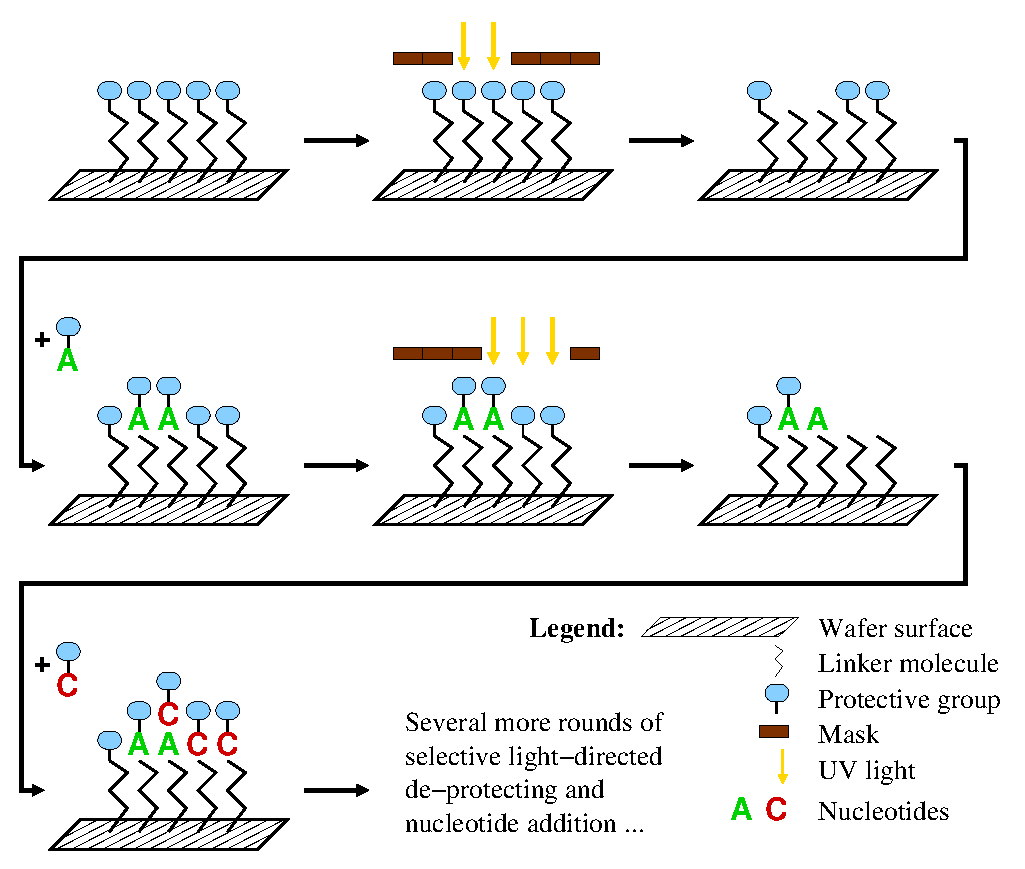
\includegraphics[width=.7\textwidth]{production.eps}
\caption{Affymetrix's probe synthesis via photolithographic masks. The chip is
  coated with a chemical compound and a light-sensitive protecting group;
  masks are used to direct light and activate selected probes for chemical
  coupling; nucleotides are appended to deprotected probes; the process is
  repeated until all probes have been fully synthesized.}
\label{fig:photolithography}
\end{figure}

Figure~\ref{fig:photolithography} illustrates this process: The quartz
wafer of a GeneChip array is initially coated with a chemical compound
topped with a light-sensitive protecting group that is removed when
exposed to ultraviolet light, activating the compound for chemical
coupling. A lithographic mask is used to direct light and remove the
protecting groups of only those positions that should receive the
nucleotide of a particular synthesis step.  A solution containing
adenine (A), thymine (T), cytosine (C) or guanine (G) is then flushed
over the chip surface, but the chemical coupling occurs only in those
positions that have been previously deprotected. Each coupled
nucleotide also bears another protecting group so that the process can
be repeated until all probes have been fully synthesized.

\subsection{Maskless Microarray Production}

Photolithographic masks are notoriously expensive and cannot be changed once
they have been manufactured. Thus, any change in the chip layout requires the
production of a new set of masks. A similar method of \emph{in situ} synthesis
known as Maskless Array Synthesizer (MAS) was later developed to eliminate the
need of such masks \citep{Singh-Gasson1999}. Probes are still built by
repeating cycles of deprotection and chemical coupling of nucleotides. The
illumination, however, relies on an array of miniature mirrors that can be
independently controlled to direct or deflect the incidence of light on the
chip.

NimbleGen Systems, Inc.\ uses its own Digital Micromirror Device (DMD) that
can control up to 786\,000 individual mirrors to produce microarrays with
spots as small as 16 $\mu$m $\times$ 16 $\mu$m. The Geniom\textR\ system of
febit biotech GmbH, a platform for customized microarray production, also uses
a micromirror array to direct the synthesis process.

\subsection{The Problem of Unintended Illumination}

Regardless of which method is used to direct light (masks or micromirror
arrays), it is possible that some probes are accidentally activated for
chemical coupling because of light diffraction, scattering or internal
reflection on the chip surface. This unwanted illumination of regions
introduces unexpected nucleotides that change probe sequences,
significantly reducing their chances of successful hybridization with their
targets. Moreover, these faulty probes may also introduce
cross-hybridizations, which can interfere in the experiments performed with
the chip.

This problem is more likely to occur near the borders between a masked and
an unmasked spot (in the case of maskless synthesis, between a spot that
is receiving light and a spot that is not). This observation has given rise to
the term \emph{border conflict}.

It turns out that by carefully designing the \emph{arrangement} of the probes
on the chip and their \emph{embeddings} (the sequences of masked and unmasked
steps used to synthesize each probe), it is possible to reduce the risk of
unintended illumination. This issue becomes even more important as there is a
need to accommodate more probes on a single chip, which requires the
production of spots at higher densities and, consequently, with reduced
distances between probes.

In this thesis, we address the problem of designing the layout of a
microarray with the goal of reducing the chances of unintended illumination,
which we call Microarray Layout Problem (MLP). We use the term \emph{layout}
to refer to where and how the probes are synthesized on the chip (their
arrangement and their embeddings).
